\section{Auswertung}
\label{sec:Auswertung}
Bevor die Langzeitmessung durchgeführt wird, werden verschieden
Bestandteile des Aufbaus kalibriert. Dazu wird die Verzögerung 
zwischen den eingehenden Signalen an der Koinzidenzschaltung 
systematisch variiert und die Impulsrate nach dieser gemessen. 
Außerdem werden Messdaten zur Kalibrierung des MCAs
aufgenommen, um einen Zusammenhang zwischen der Channelzahl und 
der Zeit zwischen Start- und Stoppsignal herstellen zu können.
\FloatBarrier
\subsection{Verzögerungszeit vor der Koinzidenzschaltung}
Die Verzögerung $\Delta t $ vor der Koinzidenzschaltung wird für 
den weiteren Versuch so gewählt, dass die 
Anzahl der Pulse nach der Schaltung (im Folgenden Counts genannt)
 maximal ist.
Die gemessenen Counts $N$ haben eine zugehörige 
Unsicherheit von $\sqrt{N}$. 
Die Messwerte sind in \autoref{tab:Verzoegerung} aufgeführt. In
der \autoref{fig:Verzoegerung} sind neben den Messwerten die
Ausgleichskonstante durch das in dem Bereich 
$\Delta t = \pm 10 \, \unit{\nano\second}$ vermutete Plateau und die 
Halbwertsbreite der Funktion dargestellt.     

\begin{table}
  \centering 
  \caption{Anzahl von der Koinzidenzschaltung ausgehende Pulse in Abhängigkeit von der Verzögerung.}
  \label{tab:Verzoegerung}
  \begin{tblr}{colspec={c c | c c}}
      \toprule
      Verzögerung $\Delta t \, [ \unit{\nano\second}]$ & Counts $N \,[\unit{\second}^{-1}]$ & Verzögerung $\Delta t \, [ \unit{\nano\second}]$ & Counts $N \, [\unit{\second}^{-1}]$\\
      \midrule
      -30 &  0,00 \pm \, 0,00 &  1 & 10,67 \pm \, 3,27 \\
      -28 &  0,00 \pm \, 0,00 &  2 & 11,80 \pm \, 3,44 \\ 
      -26 &  0,03 \pm \, 0,18 &  3 & 11,37 \pm \, 3,37 \\
      -24 &  0,00 \pm \, 0,00 &  4 &  9,30 \pm \, 3,05 \\
      -22 &  0,00 \pm \, 0,00 &  5 &  8,77 \pm \, 2,96 \\
      -20 &  0,00 \pm \, 0,00 &  6 &  7,00 \pm \, 2,65 \\
      -18 &  0,00 \pm \, 0,00 &  7 &  5,63 \pm \, 2,37 \\
      -16 &  0,03 \pm \, 0,18 &  8 &  4,03 \pm \, 2,01 \\
      -14 &  0,03 \pm \, 0,18 &  9 &  3,60 \pm \, 1,90 \\
      -12 &  0,00 \pm \, 0,00 & 10 &  2,30 \pm \, 1,52 \\
      -10 &  0,10 \pm \, 0,32 & 12 &  0,70 \pm \, 0,84 \\
      -9  &  0,23 \pm \, 0,48 & 14 &  0,23 \pm \, 0,48 \\
      -8  &  0,87 \pm \, 0,93 & 16 &  0,03 \pm \, 0,18 \\
      -7  &  1,57 \pm \, 1,25 & 18 &  0,07 \pm \, 0,26 \\
      -6  &  3,23 \pm \, 1,80 & 20 &  0,07 \pm \, 0,26 \\
      -5  &  5,03 \pm \, 2,24 & 22 &  0,03 \pm \, 0,18 \\
      -4  &  7,43 \pm \, 2,73 & 24 &  0,00 \pm \, 0,00 \\
      -3  &  8,27 \pm \, 2,88 & 26 &  0,00 \pm \, 0,00 \\
      -2  &  9,40 \pm \, 3,07 & 28 &  0,00 \pm \, 0,00 \\
      -1  & 10,93 \pm \, 3,31 & 30 &  0,00 \pm \, 0,00 \\
      0   & 11,57 \pm \, 3,40 &    &       \\
      \bottomrule
  \end{tblr}
\end{table}

Die Höhe des Plateaus beträgt $11,27 \, \sfrac{\text{Counts}}{\unit{\second}}$.
Zur Bestimmtung der Halbwertsbreite $\Delta t_{\text{HWB}}$ wird der Abstand 
beider Flanken auf halber Höhe der Ausgleichkonstanten berechnet.
Daraus ergibt sich $\Delta t_{\text{HWB}} = 11,44 \, \unit{\nano\second}$. 

Die Auflösungszeit $t_{\text{AZ}}$ wird durch  
$t_{\text{AZ}} = |2 \cdot 10 \, \unit{\nano\second}-\Delta t_{\text{HWB}}|$ berechnet.
Daraus ergibt sich $t_{\text{AZ}} = 8,56 \, \unit{\nano\second}$.

Für den weiteren Verlauf des Versuches wird eine Verzögerungszeit von $2 \,\unit{\nano\second}$ verwendet, da diese die 
größte Anzahl an Pulsen verursacht.
\begin{figure}
  \centering
  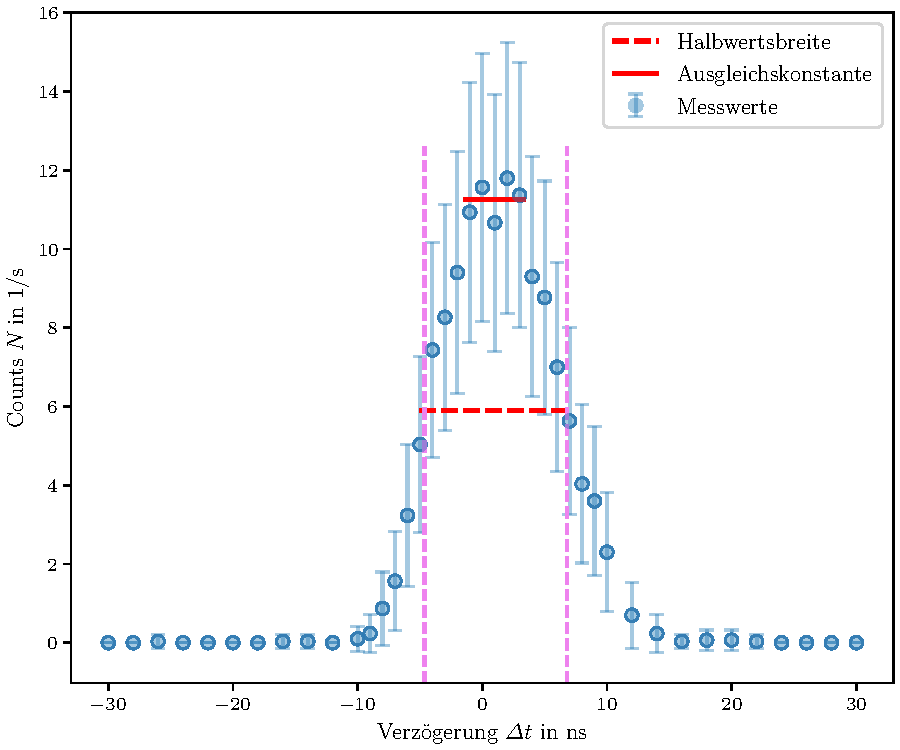
\includegraphics[width=0.75\textwidth]{Verzoegerung.pdf}
  \caption{Darstellung der Messwert der Variation der Verzögerungszeit mit Ausgleichskonstante und Bestimmung der Halbwertsbreite.}
  \label{fig:Verzoegerung}
\end{figure}
\FloatBarrier

\subsection{Kalibrierung des Multichannel-Analyzers}

Zur Kalibrierung des Multichannel-Analyzers werden die Kanäle 
gemessen, die bei verschiedenen Zeitdifferenzen befüllt werden. 
In \autoref{tab:Kalibrierung_MCA} sind die Nummern der
 gefüllten Kanäle mit der zugehörigen Zeitdifferenz 
 $\Delta t_{\text{K}}$ aufgeführt. Falls bei der gleichen Zeitdifferenz 
 mehr als ein Kanal befüllt wird, wird ein Mittelwert abhängig 
 von der Höhe der Counts in den verschiedenen Kanälen für 
 die Kanalnummer verwendet. Die Messwerte und eine lineare Regression 
 sind in \autoref{fig:Kalibrierung_MCA} graphisch dargestellt. 
 Die Ausgleichsgerade der Form $\Delta t_{\text{K}} = m \, \cdot \,\text{Kanalnummer} + n$
 stellt einen Zusammenhang zwischen Zeitdifferenz und Kanalnummer her, 
 sodass diese in einander umgerechnet werden können. 
 Aus der Augleichsrechnung ergibt sich 
 \begin{align*}
 m &= (0,0217 \pm \, 0,0000) \, \frac{\text{Counts}}{\unit{\mu\second}}\, \, \text{und} \\
 n &= (0,0965 \pm \, 0,0033) \, \unit{\mu\second} \,. 
 \end{align*}

\begin{table}
  \centering 
  \caption{Gefüllte Kanäle bei verschiedenen Zeitdifferenzen.}
  \label{tab:Kalibrierung_MCA}
  \begin{tblr}{colspec={c c | c c}}
      \toprule
      Kanalnummer & Zeitdifferenz $\Delta t_{\text{K}} \, [\unit{\mu\second}]$  & Kanalnummer & Zeitdifferenz $\Delta t_{K} \, [\unit{\mu\second}]$\\
      \midrule
      9           & 0,3 & 235         & 5,2\\
      42          & 1,0 & 267         & 5,9\\
      74          & 1,7 & 300         & 6,6\\
      106         & 2,4 & 341         & 7,5\\
      138         & 3,1 & 364         & 8,0\\
      170,69      & 3,8 & 396         & 8,7\\
      203         & 4,5 &             &    \\
      \bottomrule
  \end{tblr}
\end{table}

\begin{figure}
  \centering
  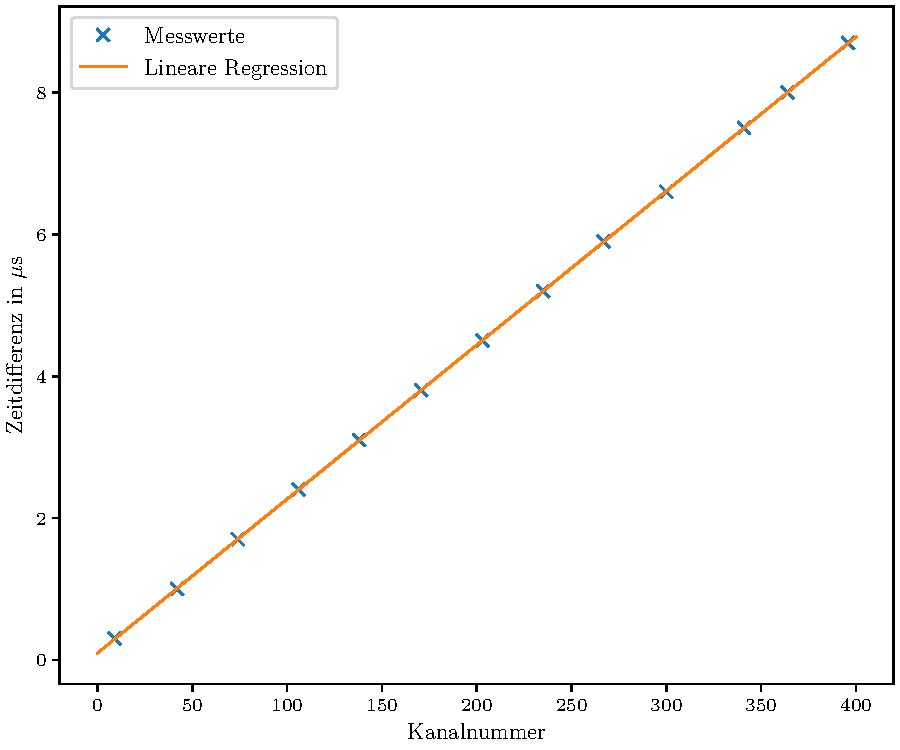
\includegraphics[width=0.75\textwidth]{Kalibrierung_MUltichannel.pdf}
  \caption{Darstellung der Messwerte der Kalibrierung des Multichannel-Analyzers mit Ausgleichsgerade.}
  \label{fig:Kalibrierung_MCA}
\end{figure}
\FloatBarrier

\subsection{Bestimmung der Lebendauer von Myonen und der Untergrundrate}
Die Lebensdauer von Myonen wird aus einer Langzeitmessung über
mehrere Tage bestimmt. 
Die aufgenommenen Messwerte sind graphisch in \autoref{fig:Lebensdauer_Myonen}
mit einer Ausgleichsfunktion dargestellt. Die Ausgleichsfunktion 
hat nach der Gleichung (\ref{eqn:Zerfallsgesetz}) die Form 
$$ N(t) = N_0 \,\symup{e}^{-\lambda t} + U \,.$$
Für die Werte ergeben sich aus der Ausgleichsrechnung 
\begin{align*}
  N_0 &= 306,8 \pm 43,8 \, ,\\
  \lambda &= (2,7618 \pm 0,2214) \frac{1}{\unit{\mu\second}} \,\, \text{und}\\
  U &= 3,77 \pm 0,53 \, .
\end{align*}

Für die Ausgleichsrechnung werden 
die ersten 16 Messwerte und die letzten 100 exkludiert. Die ersten 16
Messwerte sind ungewöhnlich niedrig für eine exponentielle Verteilung 
und die letzten 100 Kanäle enthalten keinen von 0 verschiedenen Wert. 

Die Untergrundrate entspricht dem Paramter $U$ aus der Ausgleichsfunktion 
und ist dementsprechend $$U = (3,77 \pm 0,53) \, \frac{\text{Counts}}{\text{Kanal}}\,.$$
Die Lebensdauer $\tau$ wird mithilfe von Gleichung (\ref{eqn:tau}) zu 
$\tau = (0,362 \pm 0,029) \, \unit{\mu\second} $ berechnet.

\begin{figure}
  \centering
  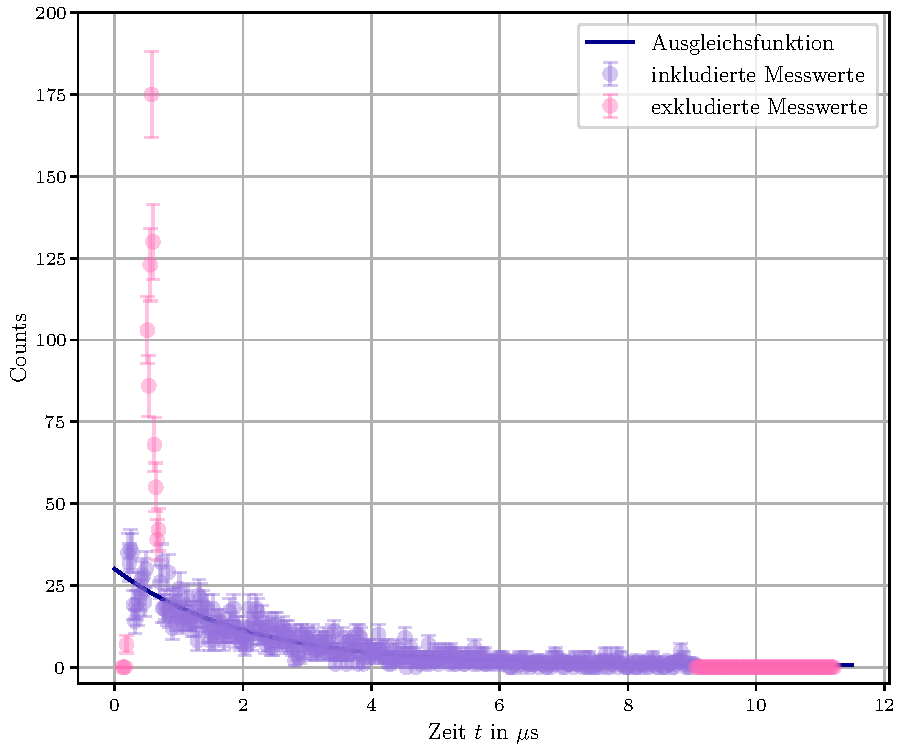
\includegraphics[width=0.70\textwidth]{Lebensdauer_der_Myonen.pdf}
  \caption{Darstellung der Messwerte zur Berechnung der Lebensdauer von Myonen mit Ausgleichsfunktion.}
  \label{fig:Lebensdauer_Myonen}
\end{figure}

%Siehe \autoref{fig:plot}!

%\begin{table}[H]
%  \centering 
%  \caption{Anzahl ausgehender Pulse in Abhängigkeit von der Verzögerung}
%  \label{tab:Verzoegerung}
%  \begin{tblr}{colspec={c c | c c}}
%      \toprule
%      Verzögerung $[\Delta t \, \unit{\nano\second}]$ & Pulsanzahl $N [1/\unit{\second}]$ & Verzögerung $[\Delta t \, \unit{\nano\second}]$ & Pulsanzahl $N [1/ \unit{\second}]$\\
%      \midrule
%      -30 &   0 0. &  1 & 320 \\
%      -28 &   0 0. &  2 & 354 \\ 
%      -26 &   1 0.03333333 &  3 & 341 \\
%      -24 &   0 0. &  4 & 297 \\
%      -22 &   0 0. &  5 & 263 \\
%      -20 &   0 0. &  6 & 210 \\
%      -18 &   0 0. &  7 & 169 \\
%      -16 &   1 0.03333333 &  8 & 121 \\
%      -14 &   1 0.03333333 &  9 & 108 \\
%      -12 &   0 0. & 10 &  69 \\
%      -10 &   3 0.1 & 12 &  21 \\
%      -9  &   7 0.23333333 & 14 &   7 \\
%      -8  &  26 0.86666667 & 16 &   1 \\
%      -7  &  47 1.56666667 & 18 &   2 \\
%      -6  &  97 3.23333333 & 20 &   2 \\
%      -5  & 151 5.03333333 & 22 &   1 \\
%      -4  & 223 7.43333333 & 24 &   0 \\
%      -3  & 248 8.26666667 & 26 &   0 \\
%      -2  & 282 9.4 & 28 &   0 \\
%      -1  & 328 10.93333333 & 30 &   0 \\
%      0   & 347 11.56666667 &    &     \\
%      \bottomrule
%  \end{tblr}
%\end{table}

%Pro Sekunde: 
%0.          
%0.          
%0.03333333  
%0.          
%0.          
%0.
%0.          
%0.03333333  
%0.03333333  
%0.          
%0.1         
%0.23333333
%0.86666667  
%1.56666667  
%3.23333333  
%5.03333333  
%7.43333333  
%8.26666667
%9.4        
%10.93333333 
%11.56666667 
%
%10.66666667 
%11.8        
%11.36666667
%9.3         
%8.76666667  
%7.          
%5.63333333  
%4.03333333  
%3.6
%2.3         
%0.7         
%0.23333333  
%0.03333333  
%0.06666667  
%0.06666667
%0.03333333  
%0.          
%0.          
%0.          
%0.    
%
%
%
%
%
%
%Fehler:
%0,00         
%0,00         
%0,18 
%0,00         
%0,00         
%0,00
%0,00         
%0,18 
%0,18 
%0,00         
%0,32 
%0,48
%0,93 
%1,25 
%1,80 
%2,24 
%2,73 
%2,88
%3,07 
%3,31 
%3,40 
%
%3,27 
%3,44 
%3,37
%3,05 
%2,96 
%2,65 
%2,37 
%2,01 
%1,90
%1,52 
%0,84 
%0,48 
%0,18 
%0,26 
%0,26
%0,18 
%0,00         
%0,00         
%0,00         
%0,00   